\lecture{Lecture - 20\hfill 14 Oct 2024, Mon}

Note that $\{1 = t^0, t, t^2, \dotsc, t^n\} = \mathcal{B},$
$\{(t)_0, (t)_1, (t)_2, \dotsc, (t)_n \} = \mathcal{C},$ and
$\{t^{(0)}, t^{(1)}, t^{(2)}, \dotsc t^{(n)}\} \- = \mathcal{D}$
form three separate bases of $\mathcal{P}_n.$



So, the formula
\begin{align*}
	t^n ={}& \sum_{k \in [n]}^{} \begin{Bmatrix} n\\k \end{Bmatrix} t^k \\
	={}& 
\end{align*}


\begin{theorem}
	If $\{ f_n \}$ and $\{g_n\}$ are sequences related by
	$$ g_n = \sum_{k=a}^{n}  \begin{Bmatrix} n\\k \end{Bmatrix} f_k,
	\qquad \forall \/ n \geq a,$$
	then we have the inversion formula
	$$ f_n = \sum_{k=a}^{n} \begin{bmatrix} n \\k \end{bmatrix}
	(-1)^{n-k} g_k, \qquad \forall \/ n \geq a.$$
\end{theorem}

\begin{remark}
	If $a=0,$ or $1,$ this follows immediately from the fact that
	$B = A^{-1}.$ Note that if $a=0,$ for $n=0,$ we have $f_0 = g_0,$
	and for $n=1,$ would imply 
	$$g_1 = \begin{Bmatrix}1\\1\end{Bmatrix} f_1, \quad
	f_1 = \begin{Bmatrix}1\\1\end{Bmatrix} g_1.$$
\end{remark}

\subsubsection*{An application to calculus}
It is easier to compute the differences between functions rather than
to compute the derivatives. In this case, we choose to approximate the
interval by a grid. A real analytic function is a smooth i.e.,
infinitely differentiable function for which the infinite Taylor Series converges about any point. For a real analytic function, $f \colon \mathbb{R} \to \mathbb{R},$ we have
\begin{align*}
	f(x+y) - f(x) ={}& y f'(x) + \frac{f^{(2)}}{2!} y^2 + \frac{f^{(3)}}{3!} y^3 + 
	\cdots\\
	={}& \sum_{k=1}^{\infty} \frac{y^k}{k!} f^{(k)}(x).
\end{align*}

In particular, if $\Delta$ represents the finite difference operator,
given by
$$(\Delta f)(x) = f(x+1) - f(x),$$
then
$$ (\Delta f)(x) = \sum_{k=1}^{\infty} \frac{f^(k)(x)}{k!} .$$


More generally, we can talk about the higher order finite difference operators such as
\begin{align*}
	( \Delta^2 f)(f) ={}& (\Delta(\Delta f))(x) \\
	={}& \Delta \left[ f(x+1) - f(x) \right] \\
	={}& \left[ f(x+2) - f(x+1) \right] - \left[ f(x+1) - f(x) \right] \\
	={}& f(x+1) - 2 f(x+1) + f(x).
\end{align*}
Similarly, we define $(\Delta^k f)(x) = (\Delta (\Delta^{k-1} f)) (x).$
\begin{theorem}
	If $f$ is real anlaytic, then
	$$ \frac{1}{k!} (\Delta ^k f)(x) = \sum_{n=k}^{\infty} 
	\frac{S(n,k)}{n!} f^{(n)} (x) .$$
	Consequently,
	$$ \frac{1}{k!} f^{(k)} (x) = \sum_{n=k}^{\infty} $$
	FILL THIS
\end{theorem}


\section{Graphs}
\begin{definition}[Adjacency Matrix]
	Given a graph $G = (V,E),$ we define its \emph{adjacency matrix} $A,$ as a matrix with rows and columns indexed by $V,$ such that
	$A(x,y)$ is the number of edges from $x$ to $y.$
\end{definition}

\begin{example}
	For the graph
	\begin{figure}[h]
	\centering
		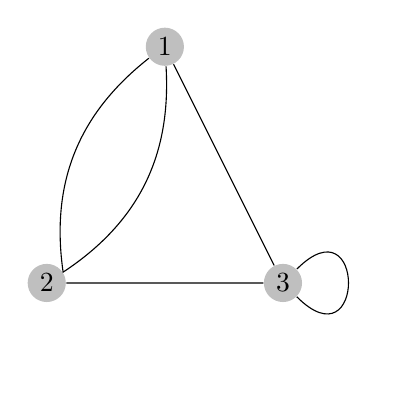
\begin{tikzpicture}
			\tikzstyle{vertex}=[circle,fill=black!25,minimum size=12pt,inner sep=2pt]
			\node[vertex] (g_1) at (3,3) {1};
			\node[vertex] (g_2) at (1.5,0) {2};
			\node[vertex] (g_3) at (4.5,0) {3};
			\draw (g_1)  to [bend left] (g_2) to [bend left]  (g_1) (g_2) -- (g_3) -- (g_1) (g_3) to [out=45, in = -45, looseness=9] (g_3);
		\end{tikzpicture}
	\end{figure}
	We have the adjacency matrix
	$\begin{bmatrix}
		0&2&1\\
		2&0&1\\
		1&1&2
	\end{bmatrix} .$
\end{example}

\begin{theorem}
	Let $G = (V,E)$ be a graph without loops and with adjacency matrix $A.$ For $x,y$ in $V,$ and any $l$ in $\mathbb{N},$ 
	$A^l(x,y)$ is the number of $(x,y)$ walks of length $l$ in $G.$
\end{theorem}

Here, $A^l(x,y)$ represents the $(x,y)^{\text{th}}$ entry of the matrix $A^l.$
